\documentclass[10pt,a4paper,]{article}
\usepackage{lmodern}
\usepackage{amssymb,amsmath}
\usepackage{ifxetex,ifluatex}
\usepackage{fixltx2e} % provides \textsubscript
\ifnum 0\ifxetex 1\fi\ifluatex 1\fi=0 % if pdftex
  \usepackage[T1]{fontenc}
  \usepackage[utf8]{inputenc}
\else % if luatex or xelatex
  \ifxetex
    \usepackage{mathspec}
  \else
    \usepackage{fontspec}
  \fi
  \defaultfontfeatures{Ligatures=TeX,Scale=MatchLowercase}
\fi
% use upquote if available, for straight quotes in verbatim environments
\IfFileExists{upquote.sty}{\usepackage{upquote}}{}
% use microtype if available
\IfFileExists{microtype.sty}{%
\usepackage{microtype}
\UseMicrotypeSet[protrusion]{basicmath} % disable protrusion for tt fonts
}{}
\usepackage[margin=1in]{geometry}
\usepackage{hyperref}
\hypersetup{unicode=true,
            pdftitle={Temperature and wave exposure as drivers of morphology in two kelp species along the coast of South Africa},
            pdfauthor={R. Coppin, C. Rautenbach, T. Ponton and A.J Smit},
            pdfborder={0 0 0},
            breaklinks=true}
\urlstyle{same}  % don't use monospace font for urls
\usepackage{longtable,booktabs}
\usepackage{graphicx,grffile}
\makeatletter
\def\maxwidth{\ifdim\Gin@nat@width>\linewidth\linewidth\else\Gin@nat@width\fi}
\def\maxheight{\ifdim\Gin@nat@height>\textheight\textheight\else\Gin@nat@height\fi}
\makeatother
% Scale images if necessary, so that they will not overflow the page
% margins by default, and it is still possible to overwrite the defaults
% using explicit options in \includegraphics[width, height, ...]{}
\setkeys{Gin}{width=\maxwidth,height=\maxheight,keepaspectratio}
\IfFileExists{parskip.sty}{%
\usepackage{parskip}
}{% else
\setlength{\parindent}{0pt}
\setlength{\parskip}{6pt plus 2pt minus 1pt}
}
\setlength{\emergencystretch}{3em}  % prevent overfull lines
\providecommand{\tightlist}{%
  \setlength{\itemsep}{0pt}\setlength{\parskip}{0pt}}
\setcounter{secnumdepth}{0}
% Redefines (sub)paragraphs to behave more like sections
\ifx\paragraph\undefined\else
\let\oldparagraph\paragraph
\renewcommand{\paragraph}[1]{\oldparagraph{#1}\mbox{}}
\fi
\ifx\subparagraph\undefined\else
\let\oldsubparagraph\subparagraph
\renewcommand{\subparagraph}[1]{\oldsubparagraph{#1}\mbox{}}
\fi

%%% Use protect on footnotes to avoid problems with footnotes in titles
\let\rmarkdownfootnote\footnote%
\def\footnote{\protect\rmarkdownfootnote}

%%% Change title format to be more compact
\usepackage{titling}

% Create subtitle command for use in maketitle
\providecommand{\subtitle}[1]{
  \posttitle{
    \begin{center}\large#1\end{center}
    }
}

\setlength{\droptitle}{-2em}

  \title{Temperature and wave exposure as drivers of morphology in two kelp
species along the coast of South Africa}
    \pretitle{\vspace{\droptitle}\centering\huge}
  \posttitle{\par}
    \author{R. Coppin, C. Rautenbach, T. Ponton and A.J Smit}
    \preauthor{\centering\large\emph}
  \postauthor{\par}
    \date{}
    \predate{}\postdate{}
  

\begin{document}
\maketitle

\hypertarget{introduction}{%
\section{Introduction}\label{introduction}}

Kelps are a group of large seaweeds of the order Laminariales
(Ochrophyta), which despite their relatively low taxonomic diversity of
species in genera (Bolton 2010), nevertheless form the basis of one of
the most productive ecosystems globally (Mann 1973). Kelps generally
have a dependence on cool, temperate and arctic seawater temperatures
(Bolton 2010; Mohring et al.~2014; Cavanaugh et al.~2011; Dayton 1985),
and dominate the nearshore biomass within the rocky shallow coasts in
both hemispheres (Steneck et al.~2002). Their size and complex
morphology provide a heterogeneous habitat structure (Steneck et
al.~2002) that accommodate a multitude of turf and subcanopy seaweed
species, and diverse assemblages of sessile and mobile invertebrates and
vertebrates (Mann 1973; Steneck et al.~2002), each depending on a wide
suite of ecological services provided by the kelp forests (Gaines \&
Roughgarden 1987; Paul \& Steneck 1993; Levin 1994; Willis \& Anderson
2003; Anderson et al.~1997; Dayton 1985). Wave exposure and temperature
are regarded as important environmental drivers of kelp forests, and
play a role in the distribution (Gorman et al.~2013), abundance
(Cavanaugh et al.~2011; Dayton et al.~1998), diversity (Wing et
al.~2007; Wernberg \& Goldberg 2008), composition (Leliaert et al.~2000;
Dayton 1985; Norderhaug et al.~2012; Harley et al.~2012), growth
(Cousens 1982) and productivity (Pedersen \& Nejrup 2012; Dayton et
al.~1998; Krumhansl \& Scheibling 2012) of kelps.

Wave exposure and temperature have also been shown to be the main
drivers of morphological adaptation across various kelp species. Past
research has shown that in highly wave exposed areas kelp morphology
tends to take on characteristics which reduce drag, increase strength
and increase flexibility (Denny \& Gaylord 2002). For example, a study
by Wernberg \& Thomsen (2005) examined the consistency of wave exposure
as a driver of \emph{Ecklonia radiata} (C. Agardh) J. Agardh across a
broad geographic range, and showed trends towards drag-reducing (small
size, narrow laterals and blades, low spinosity) and increased strength
(large holdfast, thick stipe and thick blades and lamina) at high wave
exposure sites. The morphological adaptation to wave exposure must be
kept in balance with other important processes, such as nutrient
assimilation and light absorption, which are dependent on the amount of
surface area of the blades. Therefore, there is a trade-off between
reducing overall drag and maintaining nutrient and photosynthetic
ability. Temperature has also been shown to play a role in driving kelp
morphology. For example, a study by Serisawa et al.~(2002) compared the
morphology of Ecklonia cava Kjellman growing in warm temperate and cool
temperate morphologies. The results showed that wrinkles in the blade
seem to be a characteristic of warm temperate regions. However this
study did not take into account the interaction with other environmental
variables such as wave exposure, which also affect kelp morphology. The
morphological adapatibility of kelps is driven by a combination of
environmental factors that in turn do not act independently of one
another. A study by Wernberg et al.~(2003) investigated the morphology
of \emph{E. radiata} in order to quantify the morphological variation
and whether it was dependent on spatial differences along the
Australasian coast. They found no correlation between spatial distance
and morphological similarity and rather the morphology of kelps was
representative of multiple environmental forcings on different
morphological characters at different spatial scales (Wernberg et
al.~2003). Due to the complex effects of environmental drivers on kelp
morphology, one can also expect differences in morphology between deep
and shallow water populations of the same species. Wave exposure may be
greater in shallower environments, or it may be reduced through damping
effects of kelp further offshore and natural barriers such as rock
outcrops; also, seawater temperature may be higher in shallow water
environments due to higher solar irradiance.

Other species of kelp, such as \emph{Laminaria pallida} and
\emph{Ecklonia maxima} (Osbeck) Papenfuss which are important habitat
forming seaweeds that exist around the coast of South Africa, offer a
unique opportunity to investigate the drivers of macroalgal
morphological characteristics between deep and shallow water
environments. Although both these species exist in the subtidal,
\emph{L. pallida} dominates deeper waters while \emph{E. maxima} forms
dense surface canopies in the shallower waters. Therefore, \emph{E.
maxima} is exposed to variations in wave, swell and temperature, while
\emph{L. pallida} is exposed to variations in waves and temperature.
(Molloy \& Bolton 1996) investigated the effect of depth and wave
exposure on \emph{L. pallida} at different depths and wave exposure and
showed that depth had a greater effect than wave exposure when
considering all the morphological characteristics; when considering
individual characteristics, however, wave exposure had the most
significant effect on blade thickness. Another study by Rothman et
al.~(2017) investigated the changes in morphology in shallow populations
of \emph{L. pallida} and \emph{E. maxima} along the South African
coastline and into Namibia; \emph{E. maxima} exhibited no morphological
changes along the coast but the stipes of \emph{L. pallida} become
increasingly hollow further north along the coastline. They suggested
that turbidity was the environmental driver responsible for this change.

Measures of wave exposure in ecological studies often incorporate
integrative measures of hydrodynamic conditions at a particular site
which are based on cartographical models of wave exposure.
Cartographical models of wave exposure are regarded as
`fetch-based-models' which measure the length of open water associated
with a particular site in a straight line, and are regarded as simple
measures of wave exposure. Advances in numerical modelling based on
physical/linear wave theory incorporate more complexity (wind forcing,
wave-wave interactions, wave breaking, diffraction and variation in wave
direction) into the models and allow for a quantitave, reproducible
approach for measuring wave exposure. Currently, no ecological studies
investigating macroalgal communities have incorporated 3D spectral
numerical modelling. Previous research investigating drivers of kelp
morphological characteristics used qualitative estimates of wave
exposure and did not consider other morphological characteristics.
Furthermore, only shallow populations have been considered in previous
research which ignores the effects of wave damping. No work currently
exists where other morphological characters have been considered,
quantitative estimates of environmental drivers have been calculated,
and the addition of wind as a possible driver of morphological
characteristics has been considered. The aim of this study is,
therefore, to understand how temperature, wave exposure and wind can
influence the morphology in two species of kelps around South Africa.
This will be achieved by initially understanding the variation in
temperature and waves and the consequences for morphological
characteristics of \emph{E. maxima} and \emph{L. pallida}.

\hypertarget{materials-and-methods}{%
\section{Materials and methods}\label{materials-and-methods}}

\hypertarget{site-selection}{%
\subsection{Site selection}\label{site-selection}}

Sites were chosen to represent an array of environmental gradients, as
indicated in Fig. 1. St.~Helena Bay and Betty's Bay constituted the
north western and south eastern boundary sites, respectively. These
sites are roughly 300 km apart, and lie within separate marine
provinces{[}3{]} and cover a cline in wave exposure and temperature.
Study sites span across the majority of the south-west coast, in varying
thermal and wave energy regimes. The region is dominated by kelp
communities that persist in contrasting abiotic environments. The west
coast region has been termed as a cool temperate region, which is
defined as a region where mean monthly temperatures are always above
10°C and always below 15°C (Smit et al.~2013). East of Cape Point marks
the beginning of an overlap or transition area, which is also referred
to as the Benguela-Agulhas Transition Zone (Smit et al.~2013). The
Agulhas Marine Province is characterised by a wide temperature range of
up to 7°C difference between mean monthly temperatures between summer
and winter (Smit et al.~2013). Due to the Cape Peninsula temperate
latitude, winter months bring an increased frequency of frontal
depressions that originate from the Southern Ocean (Reason et al.~2006).
These low pressures are joined by large swells with increased wave
energy. The nearshore environment, with the accompanied biota, therefore
experiences high wave energy events, with increased frequency in winter
(Veitch et al.~2018). The large peninsula acts as an obstruction for
large south westerly swells, providing decreased wave energy along the
west side of False Bay (Shipley 1964). Conversely, the west coast of
Cape Point is battered by these large swells. Multiple sites, therefore,
exist where kelps grow in diverse temperature and wave energy climates,
in close proximity.

The topography and elevation along the Cape Peninsula channel and shield
winds along False Bay. This is however absent in winter, where strong
northerly winds are prevalent from St.~Helena Bay to Betty's Bay (Field
et al.~1980; Jury et al.~1985; Andrews \& Hutchings 1980; Jury 1980).
Patterns are also evident in the wave data. Seasonal variations in
significant wave height (Hs), wave period and wave direction are also
present. The direction of the dominant swell changes to the south west
in winter, generated by strong low pressures that originate from the
southern ocean (Reason et al.~2006), which False Bay is sheltered from
(Shipley 1964; Atkins 1970; Dufois \& Rouault 2012). In summer, these
swells rotate anticlockwise and are able to enter False Bay, providing
an increased variability of Hs and Tp in this region. It should be noted
that what is classified as sheltered around the South African coastline
(a high energy coastline) might be classified as exposed in other
regions of the world (Norderhaug et al.~2012; Leliaert et al.~2000). It
is due to the near consistent south-westerly swell and the complex
orography around the peninsula that the wave energy distribution around
the Cape Peninsula varies significantly over a small geographical area.

\hypertarget{abiotic-environment}{%
\subsection{Abiotic environment}\label{abiotic-environment}}

\hypertarget{temperature}{%
\subsubsection{Temperature}\label{temperature}}

In order to compare abiotic variables for sites around the coast, large
historical databases for temperature, wave energy and wind were
accessed. Shallow water temperatures were sourced from The South African
Coastal Temperature Network (SACTN) website
(\url{https://github.com/ajsmit/SACTN}). In terms of nearshore
temperature, in situ data are preferred over satellite SST, which have
shown to exhibit large biases (Smit et al.~2013). Linear interpolated
SST were calculated for sites where \emph{in situ} recorders were
absent.

\hypertarget{wave-environment}{%
\subsubsection{wave environment}\label{wave-environment}}

Wave model variable data formed part of the South African Coastal
Vulnerability Assessment, presented to the Department of Environmental
Affairs (DEA) and produced by the Council for Scientific and Industrial
Research (CSIR) (Rautenbach 2015). The South African wave climate was
modeled via 20 spectral numerical wave models that simulated the
offshore wave climate to the nearshore. The boundary conditions of these
models were obtained by using the NOAA Wave Watch III (WWIII) model
output, distributed via the National Centers for Environmental
Prediction (NCEP) product (Office of the Director 2000; Environmental
Modeling Center / Marine Modeling Branch 2005). The particular hindcast
product utilised during the DEA-CSIR study spans 1994-2013 at a 3-hour
resolution. These data were then used to model swell propagation into
the coastal models while wind waves (seas) were generated via stationary
computations in the Simulating Waves in the Nearshore SWAN model (Booij
et al.~1997). The assumption of stationary computations are acceptable
as the model domains were small enough so the temporal variation of the
model boundary were slower than the time it takes for that boundary
condition to propagate to the coast. SWAN allows one to extract wave
variables from specific gridded locations in the nearshore. For False
Bay, a resolution of 200 meters was modelled and output produced at both
the 7 meter and 15 meter isobaths. A 200 meter resolution was used as
the False Bay computational grid was nested within a larger grid (1
kilometer resolution). This allowed for a computational effective wave
resolution of increasing resolution, from the NCEP, low resolution
output to nested, high resolution coastal output. For Table Bay and east
of Cape Hangklip the resolution was 500 meters and also had output at
the 7 meters and 15 meter isobaths. These contour outputs were chosen in
the original study by the CSIR as most engineering run-up calculations
require wave parameter information at these contour depths and were the
main focus of the original study. For this study the 7 meter contours
were used.

\hypertarget{collection-of-kelp-morphological-characteristics}{%
\subsubsection{Collection of kelp morphological
characteristics}\label{collection-of-kelp-morphological-characteristics}}

The morphological characteristics of both species are presented in Fig.
2. \emph{Laminaria pallida} is characterised by a single smooth blade
which is divided longitudinally into sections, and develops from a
single meristematic region located at the junction between the blade and
the stipe (Dyer 2018). This species has a solid stipe but develops a
hollow stipe along the west coast northward and into Namibia (Rothman et
al.~2017). \emph{Ecklonia maxima} consists of a single primary blade
which develops above a gas-filled float and a hollow stipe below.
Secondary blades are produced laterally from the primary blade from
several meristematic regions along the margins of the primary blade,
known as digits (Dyer 2018). Both species are held to the substrate by
finger-like haptera, collectively known as the holdfast.

\begin{figure}
\centering
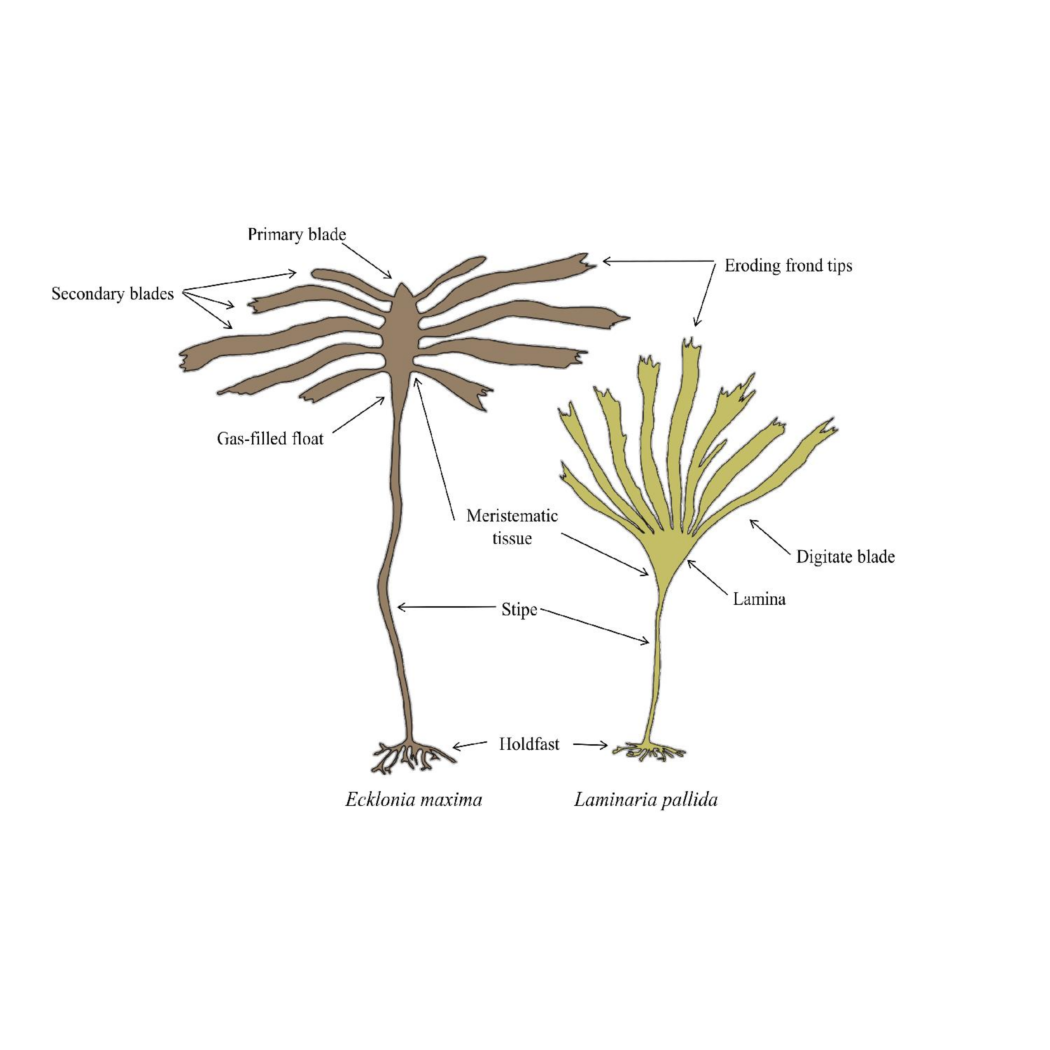
\includegraphics{paper_morph_new_files/figure-latex/unnamed-chunk-1-1.pdf}
\caption{Schematic of \emph{E. maxima} on the left and \emph{L. pallida}
on the right. (Dyer 2018)}
\end{figure}

Morphological measurements of \emph{L. pallida} and \emph{E. maxima}
were collected at 18 sites along the Western Cape coast of South Africa
(\protect\hyperlink{D2L_fig_ref_Mapux5cux2520ofux5cux2520Capeux5cux2520peninsulaux5cux2520andux5cux2520studyux5cux2520sitesux5cux2520forux5cux2520bothux5cux2520L.ux5cux2520pallidaux5cux2520andux5cux2520E.ux5cux2520maxima.ux5cux2520Theux5cux2520Redux5cux2520dotux5cux2520representsux5cux2520theux5cux2520positionux5cux2520ofux5cux2520Capeux5cux2520Townux5cux2520asux5cux2520aux5cux2520pointux5cux2520ofux5cux2520reference.}{Fig.
1}) between October 2014 and April 2015. In each instance only the
largest individuals were sampled to ensure that only mature and fully
grown sporophytes were measured. Thirteen samples were collected for
each species at each of the sites. The morphological traits named in
Tables 1 and 2 were measured for comparison between sites. Because the
macroalgae differ in morphological features, species-specific
morphological characteristics were included. This allowed comparison
between adjacent and non-adjacent sites around the peninsula. Between
February 2017 and November 2018, morphological measurements for \emph{E.
maxima} individuals in shallow water (\textless{}1m) at seven sites
along the Western Cape coast of South Africa were also collected. The
same morphological characteristic measurements were taken as for the
deeper \emph{E. maxima}, and this allowed comparison between
morphological characteristics between deep and shallow individuals
within sites. Measurements were not collected for \emph{L. pallida} in
the shallow depths, as this species is largely absent from the shallow
in this portion of the South African coastline.

\hypertarget{statisical-analyses}{%
\subsection{Statisical analyses}\label{statisical-analyses}}

Site-specific summary statistics were calculated for each of the
environmental variables considered in this study. The summary statistics
calculated for temperature, waves and wind variables were minimum,
maximum, mean, range and standard deviation for annual, February{[}6{]}
(Austral summer) and August (Austral winter) timescales, respectively.
In addition, annual and seasonal median wave and wind direction were
also calculated; all summary data and their respective abbreviation are
presented in Table 3. The median was calculated for wind and wave
direction, as issues arise when calculating the mean and standard
deviation for compass metrics. Dot and whisker plots were used to
present the summary statistics for both temperature and wave variables.
Summary statistics for wind was not plotted and instead are discussed,
as the data was course relative to the other environmental variables
considered in this study.

\emph{insert paragraph about morphology} Characterising and comparison
of morphological characteristics between deep and shallow \emph{E.
maxima} was achieved by notched boxplots. Distance-based redundancy
analysis was performed using the \emph{rda} function in the \emph{vegan}
software package \href{https://paperpile.com/c/rrvrnI/yQkq}{(Oksanen et
al.~2016)} in R (R Core Team, 2019). The role of temperature, waves and
wind as drivers of kelp morphology was investigated. The abiotic data
covered all study sites for both species of kelp. Both morphology and
abiotic data (temperature, waves and wind) were standardised using the
\emph{decostand} function in the \emph{vegan} software package;
morphology data were used as response variables and the abiotic data as
explanatory variables. To determine the explanatory variables that best
describe patterns in the response data, a full RDA was performed using a
complete set of explanatory variables. Forward selection was then used
to reduce the number of explanatory variables as well as prevent the
inflation of overall type I error
\href{https://paperpile.com/c/rrvrnI/IjDn}{(Borcard et al.~2011)}. To
further improve the model, pairwise coefficients and Variance Inflation
Factor (VIF) were calculated to identify variables with high
multicollinearity. The computation of the parsimonious RDA was followed
by permutation tests of the adjusted \emph{R}2 to assess significance of
constraints.

\hypertarget{results}{%
\section{Results}\label{results}}

\hypertarget{abiotic-environment-1}{%
\subsection{Abiotic environment}\label{abiotic-environment-1}}

The mean annual coastal water temperature for the study sites located on
the western side of the peninsula ranged from 14.5 ± 0.9 ℃ (mean ± SD)
at St.~Helena Bay, the most northern site on the western side of the
peninsula, to 14.6 ± 0.3 ℃ at Olifantsbos, the most southern site on the
western side of the peninsula. For sites located on the eastern side of
the peninsula (within False Bay), the annual mean coastal water
temperatures ranged from 15.5 ± 0.9 ℃ at Buffelsbaai to 15.0 ± 0.9 ℃ at
Betty's Bay, the most eastern site on the coastline in this study.
Oudekraal had the lowest annual mean coastal water temperature of 12.3 ±
0.9 ℃
(\protect\hyperlink{D2L_fig_ref_Temperatureux5cux2520variablesux5cux2520relativeux5cux2520toux5cux2520eachux5cux2520morphologicalux5cux2520characteristicux5cux2520collectionux5cux2520siteux5cux2520aroundux5cux2520theux5cux2520Westernux5cux2520Capeux5cux2520coast.ux5cux2520Temperatureux5cux2520parametersux5cux2520includeux5cux2520minimumux2cux5cux2520maximumux2cux5cux2520meanux2cux5cux2520rangeux5cux2520andux5cux2520standardux5cux2520deviationux5cux2520ux28ux2103ux29.ux5cux2520Forux5cux2520figuresux5cux2520inux5cux2520columnux5cux2520Aux2cux5cux2520blueux5cux2520dotsux5cux2520representux5cux2520minimumux5cux2520temperaturesux2cux5cux2520redux5cux2520representsux5cux2520maximumsux5cux2520andux5cux2520blackux5cux2520datesux5cux2520theux5cux2520meanux5cux2520temperature.ux5cux2520Errorux5cux2520barsux5cux2520representux5cux2520theux5cux2520standardux5cux2520deviation.ux5cux2520Forux5cux2520figuresux5cux2520inux5cux2520columnux5cux2520Bux2cux5cux2520blackux5cux2520dotsux5cux2520representux5cux2520temperatureux5cux2520range.ux5cux2520Temperatureux5cux2520variablesux5cux2520areux5cux2520alsoux5cux2520dividedux5cux2520intoux5cux2520Annualux5cux2520ux28topux29ux2cux5cux2520Australux5cux2520summerux5cux2520ux28middleux29ux5cux2520andux5cux2520Australux5cux2520winterux5cux2520ux28bottomux29.}{Fig.
3}), amongst all sites.

Annual maximum coastal temperatures for study sites located on the
western side of the peninsula ranged from 16.3 ℃ at St.~Helena Bay to
15.1 ℃ at Olifantsbos. For sites located east of the peninsula, annual
maximum coastal water temperatures ranged from 16 ℃ at Buffelsbaai to
16.5 ℃ at Betty's Bay. Amongst all sites, Kalk Bay had the highest
annual maximum temperature of 19 ℃. Annual minimum coastal water
temperatures for the study sites on the western side of the peninsula
ranged from 12.9 ℃ at St.~Helena Bay to 14.1 ℃ at Olifantsbos, and on
the western side of the peninsula ranged from 15.0 ℃ at Buffelsbaai to
13.6 ℃ at Betty's Bay. The annual range in temperature on the western
side on the peninsula was 3.4 at St.~Helena Bay to 0.9 at Olifantsbos,
and on the eastern side on of the peninsula was 1.0 at Buffelsbaai to
2.9 at Betty's Bay. As can be seen in Fig 3, the trend in the range of
temperature decreases from St.~Helena Bay to Miller's point and then
increases from Kalk Bay to Betty's Bay. Also, annual range in
temperatures within False Bay are larger in winter (August) compared to
summer (February).

\begin{figure}
\centering
\includegraphics{paper_morph_new_files/figure-latex/Temperature variables plot-1.pdf}
\caption{Temperature variables at the collection sites around the Cape
Peninsula. Temperature variables include minimum represented by blue
dots.}
\end{figure}

\begin{verbatim}
## Warning: Removed 3 rows containing missing values (geom_point).
\end{verbatim}

\begin{verbatim}
## Warning: Removed 3 rows containing missing values (geom_errorbar).
\end{verbatim}

\begin{verbatim}
## Warning: Removed 3 rows containing missing values (geom_point).
\end{verbatim}

\begin{verbatim}
## Warning: Removed 3 rows containing missing values (geom_errorbar).
\end{verbatim}

\begin{verbatim}
## Warning: Removed 3 rows containing missing values (geom_point).
\end{verbatim}

\begin{verbatim}
## Warning: Removed 3 rows containing missing values (geom_errorbar).
\end{verbatim}

\begin{verbatim}
## Warning: Removed 3 rows containing missing values (geom_point).
\end{verbatim}

\begin{verbatim}
## Warning: Removed 3 rows containing missing values (geom_errorbar).
\end{verbatim}

\begin{verbatim}
## Warning: Removed 3 rows containing missing values (geom_point).
\end{verbatim}

\begin{verbatim}
## Warning: Removed 3 rows containing missing values (geom_errorbar).
\end{verbatim}

\begin{verbatim}
## Warning: Removed 3 rows containing missing values (geom_point).
\end{verbatim}

\begin{verbatim}
## Warning: Removed 3 rows containing missing values (geom_errorbar).
\end{verbatim}

\begin{figure}
\centering
\includegraphics{paper_morph_new_files/figure-latex/wave variable plot-1.pdf}
\caption{Wave variables at each collection site around the Western Cape
coast. Mean variables are represented by dots and standard deviation by
whiskers.}
\end{figure}

Our data show the western side of the peninsula experiences higher
significant wave heights and variation in wave heights compared to the
eastern side of the peninsula on both an annual and seasonal scale.
Annual mean significant wave height ranged from 0.5 ± 0.2 m (mean ± SD)
at St.~Helena Bay to 2.3 ± 0.7 m at Olifantsbos on the western side of
the peninsula, and on the eastern side of the peninsula it ranged from
0.9 ± 0.4 m at Buffelsbaai to 1.9 ± 0.6 m at Betty's Bay
(\protect\hyperlink{D2L_fig_ref_ux5cux2520Waveux5cux2520parametersux5cux2520relativeux5cux2520toux5cux2520eachux5cux2520morphologicalux5cux2520characteristicux5cux2520collectionux5cux2520siteux5cux2520aroundux5cux2520theux5cux2520Westernux5cux2520Capeux5cux2520coast.ux5cux2520Variablesux5cux2520areux5cux2520colourux5cux2520codedux2cux5cux2520plotsux5cux2520withux5cux2520blueux5cux2520dotsux5cux2520representux5cux2520significantux5cux2520waveux5cux2520heightux5cux2520ux28metersux29ux5cux2520andux5cux2520theux5cux2520associatedux5cux2520standardux5cux2520deviationux2cux5cux2520andux5cux2520plotsux5cux2520withux5cux2520redux5cux2520dotsux5cux2520representux5cux2520significantux5cux2520waveux5cux2520periodux5cux2520ux28secondsux29ux5cux2520andux5cux2520theux5cux2520associatedux5cux2520standardux5cux2520deviation.ux5cux2520Plotsux5cux2520withux5cux2520blackux5cux2520dotsux5cux2520representux5cux2520waveux5cux2520directionux5cux2520ux28bearingux29.ux5cux2520Waveux5cux2520variablesux5cux2520dividedux5cux2520intoux5cux2520Annualux5cux2520ux28topux29ux2cux5cux2520Australux5cux2520summerux5cux2520ux28middleux29ux5cux2520andux5cux2520Australux5cux2520winterux5cux2520ux28bottomux29ux5cux2520respectively.}{Fig.
4}). The annual maximum significant wave height ranged from 1.4 m at
St.~Helena Bay to 4.7 m at Olifantsbos on the western side of the
peninsula, and on the eastern side ranged from 2.6 m at Buffelsbaai to
4.2 m at Betty's Bay. These wave heights and their variability are
modulated by the relative sheltering against the predominant
south-westerly swell direction and the size of the fetch for local wave
generation.

Annual mean wave peak period for sites on the western side of the
peninsula ranged from 10.3 ± 3.5 s at St.~Helena Bay to 11.0 ± 2.0 s at
Olifantsbos, and ranged from 10.6 ± 3.0 s at Buffelsbaai to 10.8 ± 2.2 s
at Betty's Bay
(\protect\hyperlink{D2L_fig_ref_ux5cux2520Waveux5cux2520parametersux5cux2520relativeux5cux2520toux5cux2520eachux5cux2520morphologicalux5cux2520characteristicux5cux2520collectionux5cux2520siteux5cux2520aroundux5cux2520theux5cux2520Westernux5cux2520Capeux5cux2520coast.ux5cux2520Variablesux5cux2520areux5cux2520colourux5cux2520codedux2cux5cux2520plotsux5cux2520withux5cux2520blueux5cux2520dotsux5cux2520representux5cux2520significantux5cux2520waveux5cux2520heightux5cux2520ux28metersux29ux5cux2520andux5cux2520theux5cux2520associatedux5cux2520standardux5cux2520deviationux2cux5cux2520andux5cux2520plotsux5cux2520withux5cux2520redux5cux2520dotsux5cux2520representux5cux2520significantux5cux2520waveux5cux2520periodux5cux2520ux28secondsux29ux5cux2520andux5cux2520theux5cux2520associatedux5cux2520standardux5cux2520deviation.ux5cux2520Plotsux5cux2520withux5cux2520blackux5cux2520dotsux5cux2520representux5cux2520waveux5cux2520directionux5cux2520ux28bearingux29.ux5cux2520Waveux5cux2520variablesux5cux2520dividedux5cux2520intoux5cux2520Annualux5cux2520ux28topux29ux2cux5cux2520Australux5cux2520summerux5cux2520ux28middleux29ux5cux2520andux5cux2520Australux5cux2520winterux5cux2520ux28bottomux29ux5cux2520respectively.}{Fig.
4}). The data shows no trend in mean peak wave period for the coastline.
Annual peak wave period was 10.0 ± 3.0 s and 9.2 ± 3.1 s in winter and
summer respectively, Miller's point and had the lowest peak wave period
amongst all sites. These data show that the western side of the
peninsula has a lower variation (SD) compared to the eastern side of the
peninsula, with Miller's point showing the highest variation across
timescales. Annual maximum peak wave period ranged from 18.9 s at
St.~Helena Bay to 18.4 s at Olifantsbos for the western side of the
peninsula, and ranged from 18.0 s at Buffelsbaai to 18.0 s at Betty's
Bay on the eastern side of the peninsula. Data for median wave direction
showed no trend across timescales; however the variation (SD) in wave
direction is lower on the western side of the peninsula compared to the
eastern side both annually and for winter. Summer data were the
exception and showed lower variation for the eastern side of the
peninsula
(\protect\hyperlink{D2L_fig_ref_ux5cux2520Waveux5cux2520parametersux5cux2520relativeux5cux2520toux5cux2520eachux5cux2520morphologicalux5cux2520characteristicux5cux2520collectionux5cux2520siteux5cux2520aroundux5cux2520theux5cux2520Westernux5cux2520Capeux5cux2520coast.ux5cux2520Variablesux5cux2520areux5cux2520colourux5cux2520codedux2cux5cux2520plotsux5cux2520withux5cux2520blueux5cux2520dotsux5cux2520representux5cux2520significantux5cux2520waveux5cux2520heightux5cux2520ux28metersux29ux5cux2520andux5cux2520theux5cux2520associatedux5cux2520standardux5cux2520deviationux2cux5cux2520andux5cux2520plotsux5cux2520withux5cux2520redux5cux2520dotsux5cux2520representux5cux2520significantux5cux2520waveux5cux2520periodux5cux2520ux28secondsux29ux5cux2520andux5cux2520theux5cux2520associatedux5cux2520standardux5cux2520deviation.ux5cux2520Plotsux5cux2520withux5cux2520blackux5cux2520dotsux5cux2520representux5cux2520waveux5cux2520directionux5cux2520ux28bearingux29.ux5cux2520Waveux5cux2520variablesux5cux2520dividedux5cux2520intoux5cux2520Annualux5cux2520ux28topux29ux2cux5cux2520Australux5cux2520summerux5cux2520ux28middleux29ux5cux2520andux5cux2520Australux5cux2520winterux5cux2520ux28bottomux29ux5cux2520respectively.}{Fig.
4}). This phenomenon can be explained by the sheltering effect of the
Cape Peninsula, resulting in a wave climate with a narrower directional
spreading on the eastern side of the peninsula (refer to Fig. 7).

In Figure 5 the total coastal wave exposure of the Cape Peninsula is
given in terms of wave energy (kW per meter wave crest length). The
directional sheltering effect of the Cape Peninsula, against the
dominant swell direction is clearly observed in the wave exposures
presented in {[}Fig. 6{]}(\#D2L\_fig\_ref\_The total and seasonal wave
roses of the directional wave buoy just offshore from Cape Town is given
form the years 2000 till end 2017 (the period for which directional wave
spectra was available.). The classification from fully sheltered to
extremely exposed is based on the total wave energy upper and lower
limits. The western periphery of the Cape peninsula is almost
continuously exposed to high wave exposures while the eastern periphery
of the peninsula (western coastline of False Bay) revealed sheltered
wave exposures {[}Fig. 6{]}(\#D2L\_fig\_ref\_The total and seasonal wave
roses of the directional wave buoy just offshore from Cape Town is given
form the years 2000 till end 2017 (the period for which directional wave
spectra was available.). Here the marked seasonality, with higher energy
waves during winter, may be clearly observed once more. To clarify the
averaged wave exposure maps presented, the propagation of a typical
offshore wave spectrum as produced from a single time-step in SWAN is
presented in
\protect\hyperlink{D2L_fig_ref_Theux5cux2520propagationux5cux2520ofux5cux2520aux5cux2520typicalux5cux2520offshoreux5cux2520waveux5cux2520spectrumux5cux2520isux5cux2520givenux5cux2520asux5cux2520producedux5cux2520fromux5cux2520aux5cux2520singleux5cux2520time-stepux5cux2520inux5cux2520SWAN}{Fig.
7}. Tracing the wave height contours into False Bay its clear why this
bay's western periphery is predominantly sheltered. It should be
mentioned that some of the annual winter frontal depression systems pass
the Cape Peninsula from the west to east, resulting in wave propagating
towards the continent from much more southerly directions. This results
in positive and negative wave exposure anomalies all around the
peninsula.

\hypertarget{drivers-of-kelp-morphological-characteristics}{%
\subsection{Drivers of kelp morphological
characteristics}\label{drivers-of-kelp-morphological-characteristics}}

\includegraphics{paper_morph_new_files/figure-latex/laminaria plots-1.pdf}
\includegraphics{paper_morph_new_files/figure-latex/laminaria plots-2.pdf}

\includegraphics{paper_morph_new_files/figure-latex/deep ecklonia plots-1.pdf}
\includegraphics{paper_morph_new_files/figure-latex/deep ecklonia plots-2.pdf}

\includegraphics{paper_morph_new_files/figure-latex/shallow ecklonia temp plots-1.pdf}
\includegraphics{paper_morph_new_files/figure-latex/shallow ecklonia temp plots-2.pdf}


\end{document}
